% tikz picture giving vector row-product illustration.
%
\usetikzlibrary{matrix,shapes,arrows}
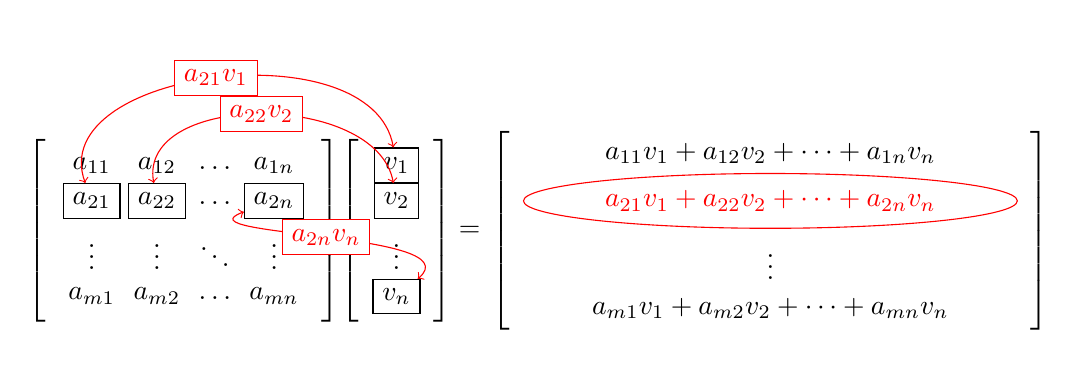
\begin{tikzpicture}
% les matrices
\matrix (A) [matrix of math nodes,%
             nodes = {},%
             left delimiter  = {[},%
             right delimiter = {]}] at (0,0)
{%
  a_{11} & a_{12} & \ldots & a_{1n}  \\
  \node[draw] (A21) {a_{21}};%
         & \node[draw] (A22) {a_{22}};%
                  & \ldots%
                           & \node[draw] (A2n) {a_{2n}}; \\
  \vdots & \vdots & \ddots & \vdots  \\
  a_{m1} & a_{m2} & \ldots & a_{mn}  \\
};
v\matrix (v) [xshift=1cm,matrix of math nodes,nodes = {},% 
              left delimiter  = [,right delimiter ={]}] at (A.east)
{%
  \node[draw] (v1)  {v_1};\\
  \node[draw] (v2) {v_2};\\
                       \vdots \\
  \node[draw] (vn) {v_n};\\
};
\node[circle,xshift=0.5cm] (E) at (v.east) {$=$}; 
w\matrix (w) [xshift=3.5cm,%
             matrix of math nodes,%
             nodes = {},%
             left delimiter  = [,%
             right delimiter ={]}] at (E.east)
{%
  a_{11}v_1+a_{12}v_2+\cdots+a_{1n}v_n\\\\
  \node[draw,ellipse,red] (X) {a_{21}v_1+a_{22}v_2+\cdots+a_{2n}v_n};\\
  \vdots \\
  a_{m1}v_1+a_{m2}v_2+\cdots+a_{mn}v_n\\
};
\draw[<->,red](A21) to[in=100,out=110]
node[draw,midway,fill=white] (x) {$a_{21}v_{1}$} (v1);
\draw[<->,red](A22) to[in=100,out=100]
node[draw,midway,fill=white] (y) {$a_{22}v_{2}$} (v2);
\draw[<->,red](A2n) to[in=400,out=200]
node[draw,midway,fill=white] (z) {$a_{2n}v_{n}$} (vn);
%\draw[-,blue] (x) to node[draw,midway,fill=white] (Y) {$+$} (y);
%\draw[-,blue] (y) to node[draw,midway,fill=white] (Z) {$\vdots$}  (z);
\end{tikzpicture}

